\documentclass{article}
\usepackage{tikz}
\usepackage{geometry}
\usepackage{pgfgantt}
\geometry{legalpaper,margin=0.75in,paperheight=6in,paperwidth=14in}

\begin{document}

\centering
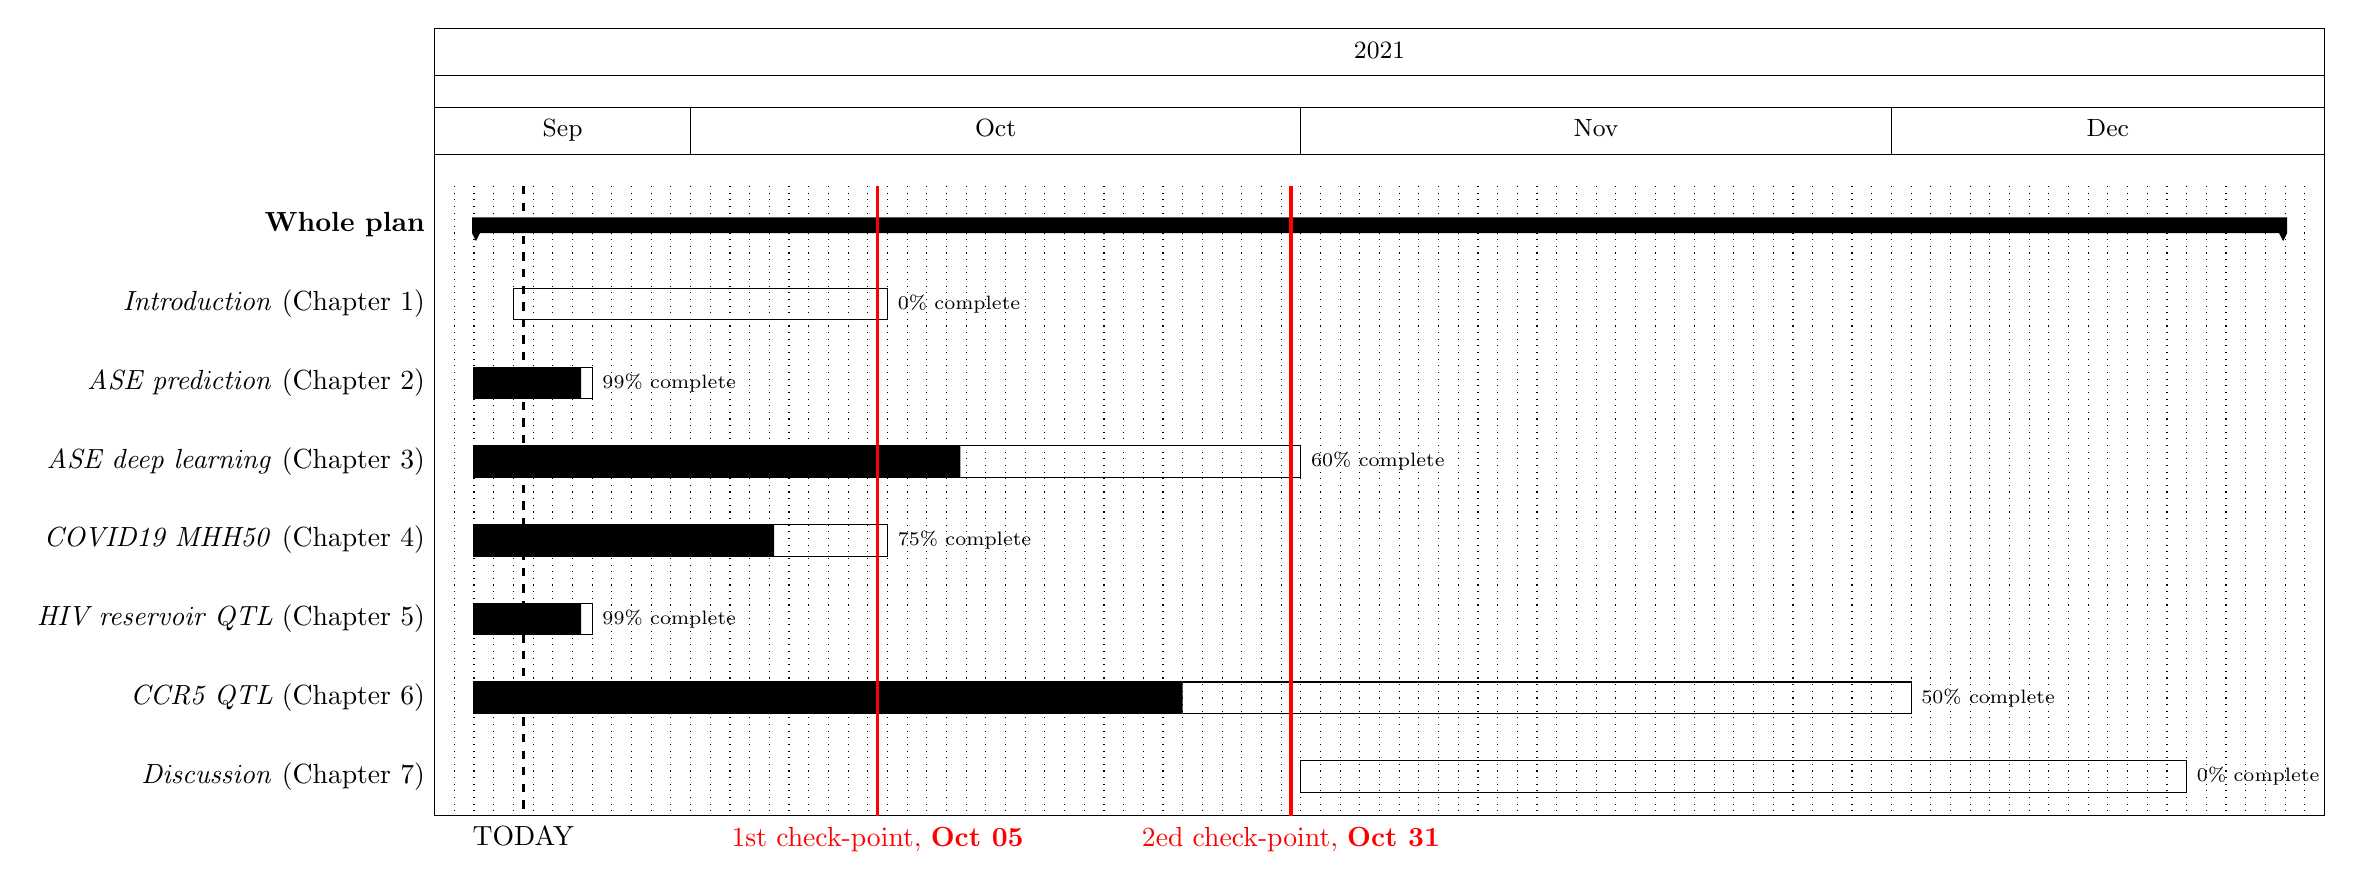
\begin{tikzpicture}
\begin{ganttchart}[
  vgrid,
  %hgrid,
  x unit=2.5mm, % cell width
  time slot format=isodate,
  today=2021-09-22,
  today offset=0.5,
  vrule offset=0.5,
  vrule/.style={very thick, red},
  bar/.append style={fill=black},
  bar incomplete/.append style={fill=none}
  ]{2021-09-18}{2021-12-22}
  \gantttitlecalendar{year,month=shortname} \\
  \ganttgroup{Whole plan}{2021-09-20}{2021-12-20} \\
  \ganttbar[progress=0]{\textit{Introduction} (Chapter 1)}{2021-09-22}{2021-10-10} \\
  \ganttbar[progress=99]{\textit{ASE prediction} (Chapter 2)}{2021-09-20}{2021-09-25} \\
  \ganttbar[progress=60]{\textit{ASE deep learning} (Chapter 3)}{2021-09-20}{2021-10-31} \\
  \ganttbar[progress=75]{\textit{COVID19 MHH50} (Chapter 4)}{2021-09-20}{2021-10-10} \\
  \ganttbar[progress=99]{\textit{HIV reservoir QTL} (Chapter 5)}{2021-09-20}{2021-09-25} \\
  \ganttbar[progress=50]{\textit{CCR5 QTL} (Chapter 6)}{2021-09-20}{2021-12-01} \\
  \ganttbar[progress=0]{\textit{Discussion} (Chapter 7)}{2021-11-01}{2021-12-15}
  \ganttvrule{1st check-point, \textbf{Oct 05}}{2021-10-10}
  \ganttvrule{2ed check-point, \textbf{Oct 31}}{2021-10-31}
\end{ganttchart}
\end{tikzpicture}

\end{document}
